\documentclass[dvipsnames]{article}
\usepackage[utf8]{inputenc}
\usepackage[english]{babel}
\usepackage[doublespacing]{setspace}
\usepackage[mathlines]{lineno}
\usepackage{minted}
\usepackage{numprint}
\usepackage{csquotes,xpatch}
\usepackage{fancyhdr,lipsum}
\usepackage{amsmath}
\usepackage{amsfonts}
\usepackage[normalem]{ulem}
\usepackage[color=blue!30!white,textsize=small,textwidth=30mm]{todonotes}
\usepackage[left=2cm,top=2cm,right=3.5cm,bottom=2cm,bindingoffset=0.5cm]{geometry}
\usepackage{bm}
%\linenumbers
\pagenumbering{arabic}

\usepackage{tabularray}
\usepackage{codehigh}
\UseTblrLibrary{booktabs}
\UseTblrLibrary{siunitx}
\newcommand{\tinytableTabularrayUnderline}[1]{\underline{#1}}
\newcommand{\tinytableTabularrayStrikeout}[1]{\sout{#1}}
\NewTableCommand{\tinytableDefineColor}[3]{\definecolor{#1}{#2}{#3}}


%TC:incbib

%%%%% For title page:
\usepackage{authblk}
\title{Title: something about recombination, genomic prediction and fitness}
\author[1,2,*]{Kenneth Aase}
\author[...]{...}
\author[2,3]{Henrik Jensen}
\author[1,2]{Stefanie Muff}
\author[4]{Susan Johnston}
\affil[1]{Department of Mathematical Sciences, Norwegian University of Science and Technology, Trondheim, Norway}
\affil[2]{The Gjærevoll Centre, Norwegian University of Science and Technology, Trondheim, Norway}
\affil[3]{Department of Biology, Norwegian University of Science and Technology, Trondheim, Norway}
\affil[4]{Edin, Edin, Edin}
\affil[*]{Corresponding author: Kenneth Aase, kenneth.aase@ntnu.no}
\date{}

%%%%% Running headline:
\renewcommand\rightmark{Short Title here}

%%%%% Bibliography
\usepackage{natbib}
\newcommand*{\citef}[1]{\footnote{\cite{#1}}}
%\usepackage[
%backend=biber,
%style=chicago-authordate,
%citestyle=authoryear,
%maxnames = 2,
%date=long,
%useprefix=true,
%sortlocale=norwegian,
%dateabbrev=false
%uniquename=false
%]{biblatex}

%\usepackage[style=authoryear, backend=biber, bibencoding=inputenc]{biblatex}
%\addbibresource{mylib.bib}
%\uspunctuation

%%%% Custom commands
\newcommand{\E}{\mathsf{E}}
\newcommand{\Prob}{\mathsf{P}}
\newcommand{\Var}{\mathsf{Var}}
\newcommand{\Cov}{\mathsf{Cov}}
\newcommand{\Corr}{\mathsf{Corr}}
\newcommand\given[1][]{\:#1\vert\:}
\newcommand{\N}[2]{\mathsf{N}\left(#1, #2\right)}
\newcommand*\diff{\mathop{}\!\mathrm{d}}
\newcommand{\ie}{\emph{i.e.}}
\newcommand{\eg}{\emph{e.g.}}
\newcommand{\Ie}{\emph{I.e.}}
\newcommand{\Eg}{\emph{E.g.}}
\newcommand{\note}[1]{\textcolor{red}{\scriptsize #1}}
\newcommand{\hl}{\textcolor{blue}}

% Table settings
\usepackage{booktabs}
\usepackage{multirow}
\usepackage{color, colortbl}
\newcommand{\ra}[1]{\renewcommand{\arraystretch}{#1}}
\definecolor{DarkGray}{gray}{0.8}
\definecolor{LightGray}{gray}{0.925}

% For figures and tables

\usepackage{graphicx}
\usepackage{cprotect}
\usepackage{float}
\floatstyle{plain}
\restylefloat{figure}
\floatstyle{plaintop}
\restylefloat{table}

\usepackage{caption} 
%\captionsetup[table]{skip=pt}

\usepackage[pdftex,bookmarks=true,hidelinks]{hyperref}
\hypersetup{
    %colorlinks=true,
    linkcolor=blue
}

% \renewcommand{\thetable}{S\arabic{table}}
% \renewcommand{\thefigure}{S\arabic{figure}}

\usepackage{verbatim}

\newcommand{\detailtexcount}[1]{%
  \immediate\write18{texcount -merge -sum -q #1.tex output.bbl > #1.wcdetail }%
  \verbatiminput{#1.wcdetail}%
}

\newcommand{\quickwordcount}[1]{%
  \immediate\write18{texcount -1 -sum -merge -q #1.tex output.bbl > #1-words.sum }%
  \input{#1-words.sum} words%
}

\newcommand{\quickcharcount}[1]{%
  \immediate\write18{texcount -1 -sum -merge -char -q #1.tex output.bbl > #1-chars.sum }%
  \input{#1-chars.sum} characters (not including spaces)%
}
\begin{document}

%%%% Comment in/out different .tex files to compile/include them or not

%TC:ignore
\maketitle
\newpage

\section*{Introduction}

\section*{Methods}

\subsection*{Data}

…

\subsection*{Genomic Prediction}

Given measurements of the crossover count $y_{ij}$ of individual $i$ (estimated from offspring $j$) we model
\begin{equation*}
    y_{ij} = \alpha + \beta_\text{coverage} \cdot \text{coverage}_{ij} + g_i + \text{hy}_i + \text{hi}_i + \text{id}_i + \varepsilon_{ij}
\end{equation*}

Although the crossover count $y_{ij}$ is a count we treat it as a continuous Gaussian

priors on random effects: $PC(var = \hat{\sigma}^2_y / 2, 0.05)$ 

Fitting the GP model results in marginal posterior distributions for each breeding value. All of which approximately normal (can show by looking at QQ plots), so we can write
\begin{equation*}
    g_i \sim N(\mu_i, \sigma_i^2)
\end{equation*}

\subsection*{Fitness analyses}

We investigate the impact of the breeding values for sex-specific breeding values on fitness components.

% Sentences Susan asked for:
The Bayesian genomic prediction model gives us a full posterior for each individual breeding value $g_i$. 
In the fitness models, we can therefore incorporate the measurement error in these breeding value by sampling breeding values from these posterior distributions. 
Rather than treating the breeding values as having fixed, known values, we sample each breeding value $g_i$ in each MCMC iteration, and regress on these samples (and their square) in the logistic regression. 
(This is equivalent to assuming a Berkson measurement error model for the breeding values.)

\subsubsection*{Annual survival}

For individual $i$ in year $j$ we model the survival as a logistic GLMM, written here as a Bayesian hierarchical model:
\begin{align*}
    &g_i \sim N(\mu_i, \sigma_i^2) \\
    &\eta_{ij} = \alpha + \beta_g \cdot g_i + beta_{g^2} \cdot g_i^2 + \beta_\text{age} \cdot \text{age} + \beta_{\text{age}^2} \cdot \text{age}^2 + \beta_f \cdot f + \text{isl}_i + \text{year}_? + \text{id}_i + \varepsilon_{ij}\\
    &P(\text{survival}_{ij} = 1) = \text{logit}^{-1}(\eta_{ij})
\end{align*}


\subsubsection*{Annual reproductive success}

...

\section*{Results}

\begin{figure}
    \centering
    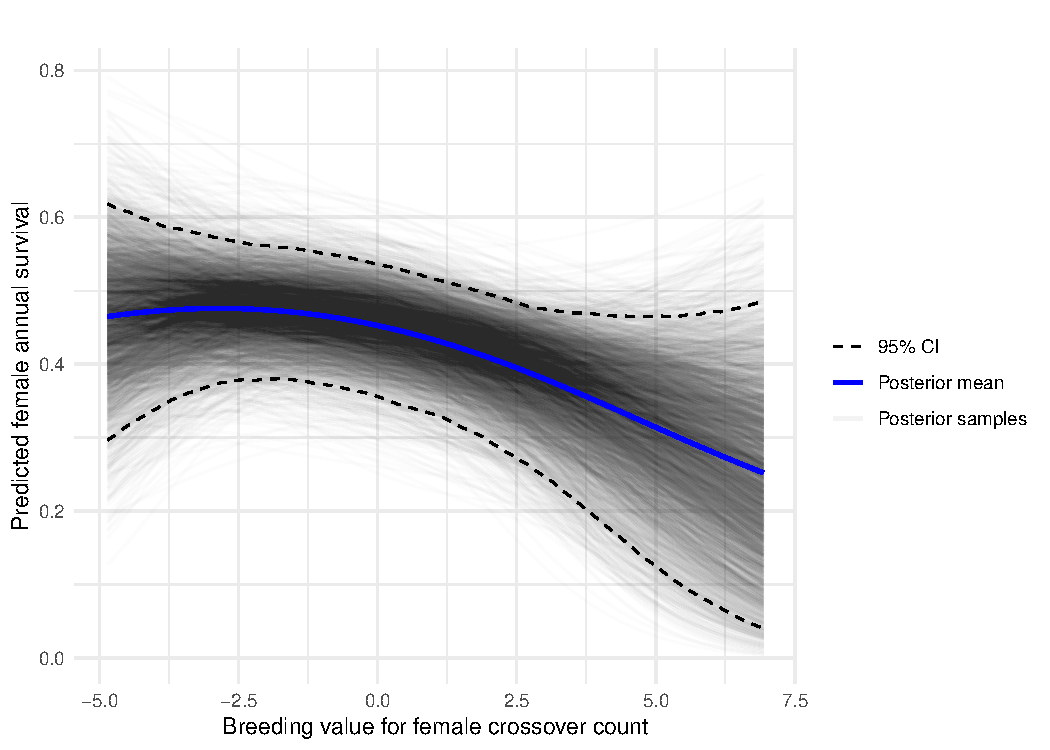
\includegraphics[width=0.91\linewidth]{figs/surv_bv_pred_f.pdf}
    \caption{...}
    \label{fig-surv_bv_f}
\end{figure}

\begin{figure}
    \centering
    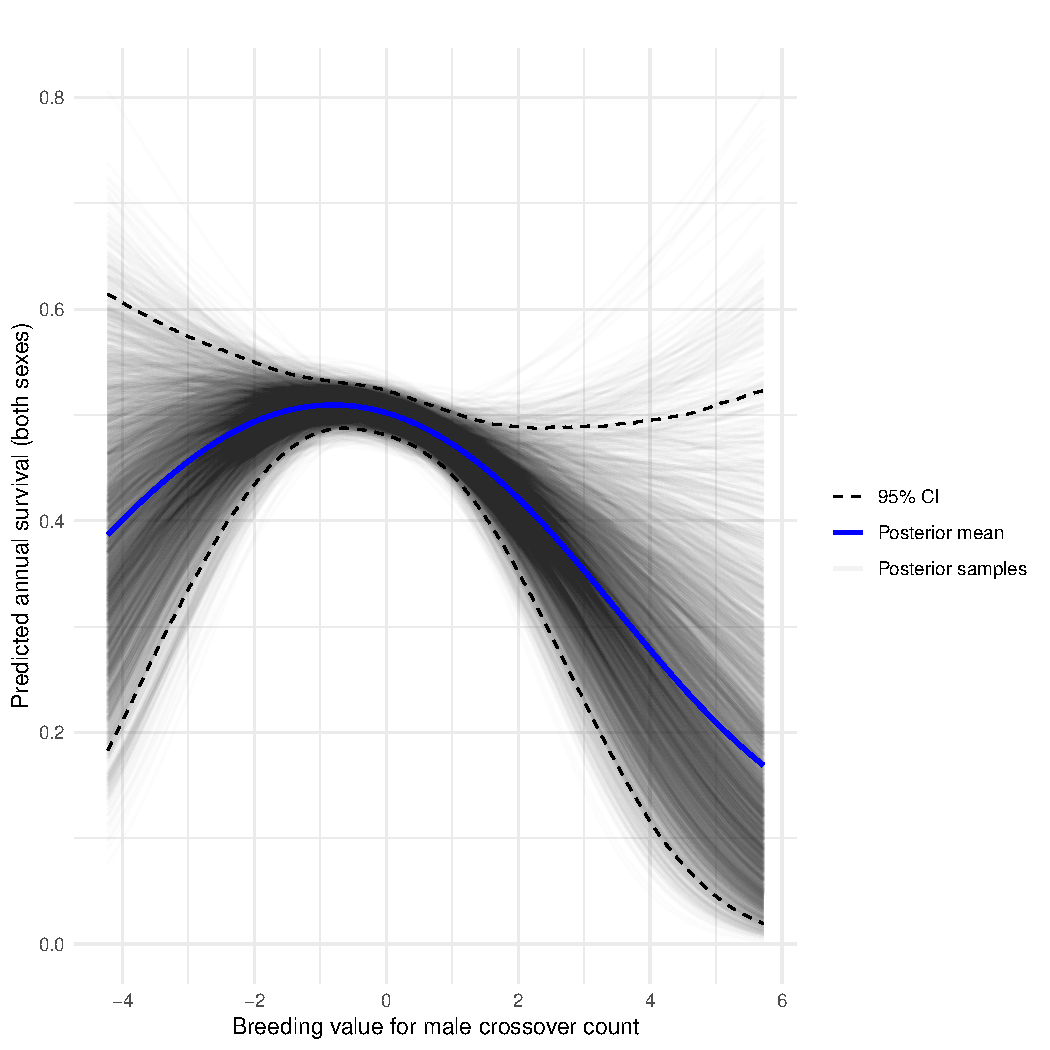
\includegraphics[width=0.91\linewidth]{figs/surv_bv_pred_m.pdf}
    \caption{...}
    \label{fig-surv_bv_m}
\end{figure}

\section*{Discussion}

\end{document}